\section{W-Algebras as $A_\infty$ Chiral Algebras: Virasoro and $W_3$}
% label removed: sec:W-algebras

This section works out W-algebra examples in the framework of $A_\infty$ chiral algebras via the Khan--Zeng 3D holomorphic-topological Poisson sigma model \cite{KZ25}. We compute:
\begin{enumerate}[label=(\roman*)]
\item The 3D HT gauge theory action for W-type PVAs;
\item Explicit propagators and $\lambda$-brackets $m_2$;
\item Higher $A_\infty$ operations $m_k$ up to $k=7$ via Feynman diagrams;
\item Generating functions encoding all $m_k$;
\item Spectral $r$-matrices and quantization data;
\item Chiral Hochschild cochains and deformation theory.
\end{enumerate}

W-algebras are higher-spin extensions of the Virasoro algebra, arising from 3D higher-spin gravity. Their non-formality and quantum corrections make them test cases for the $d'=1$ regime.

\subsection{General Framework: PVA to 3D HT Gauge Theory}
% label removed: subsec:PVA-to-3DHT

\subsubsection{The Khan--Zeng Construction}

Let $\mathcal{V} = \Sym(\C[\partial]\langle \phi^i \rangle)$ be a freely generated Poisson vertex algebra with generators $\phi^i$ of conformal spins $s_i$. The $\lambda$-bracket
\[
\{\phi^i{}_\lambda \phi^j\} = \sum_{n \geq 0} \Pi^{ij}_n \lambda^n, \quad \Pi^{ij}_n \in \mathcal{V},
\]
encodes the classical Poisson structure. 

\begin{construction}[3D HT Poisson Sigma Model]
% label removed: const:3d-poisson-sigma
To each PVA $\mathcal{V}$, Khan and Zeng associate a 3D holomorphic-topological gauge theory on $\R \times \C$ with fields:
\begin{itemize}
\item $\Phi^i = \phi^i_{zz\cdots z}(t,z,\bar{z})(dz)^{\otimes s_i}$, the holomorphic field of spin $s_i$;
\item $\eta_i = (\eta_i^t dt + \eta_i^{\bar{z}} d\bar{z}) \otimes (dz)^{\otimes(1-s_i)}$, the Lagrange multiplier (conjugate momentum) of spin $1-s_i$.
\end{itemize}
The action functional is
\begin{equation}
% label removed: eq:KZ-action
S = \int_{\R \times \C} \eta_i (d_t + \bar{\partial})\Phi^i + \frac{1}{2} \eta_i \Pi^{ij}(\partial_z) \eta_j,
\end{equation}
where $\Pi^{ij}(\partial) = \sum_n \Pi^{ij}_n \partial^n$ is the differential operator encoding the $\lambda$-bracket.

The gauge transformations are
\begin{align}
\delta \Phi^i &= \Pi^{ij}(\partial) \epsilon_j,\\
\delta \eta_i &= -(d_t + \bar{\partial})\epsilon_i - \eta_j \frac{\partial \Pi^{jk}}{\partial \Phi^i}(\partial) \epsilon_k,
\end{align}
where $\epsilon_i$ are gauge parameters of spin $1-s_i$.
\end{construction}

\begin{remark}[Higher-Spin Gravity]
When $\mathcal{V}$ is a W-algebra, the resulting 3D theory is a form of higher-spin gravity in the sense of Henneaux--Teitelboim and Vasiliev. The gauge symmetry extends diffeomorphisms to include higher-spin transformations.
\end{remark}

\subsubsection{BV Quantization and $A_\infty$ Operations}

\begin{remark}[Analytic hypotheses for W-algebra examples]
% label removed: rem:W-hypotheses
All results in this section are conditional on Hypotheses~\ref{hyp:H1}--\ref{hyp:H3} and Assumption~\ref{ass:H1-H4}. Verification proceeds as follows.
\emph{(H1)}: The BV data for the Khan--Zeng 3D HT Poisson sigma model is constructed explicitly; one-loop finiteness follows from the holomorphic structure by the arguments of \cite{GRW21,GGW21}.
\emph{(H2)}: The propagator $K(t,z) = \Theta(t)/(2\pi z)$ is meromorphic in $z$ with a simple pole and has step-function (exponential) decay in $t$, satisfying the required regularity.
\emph{(H3)}: The interaction vertices are polynomial in fields and derivatives, so the configuration-space integrals defining $m_k$ converge on $\FM_k(\C) \times \Conf_k(\R)$ by standard estimates; the AOS relations hold on logarithmic forms.
\emph{(H4)}: Factorization compatibility follows from the general construction of \cite{CDG20,GKW25} for HT gauge theories with polynomial interactions.
\end{remark}

In the BV formalism, we introduce antifields $(\Phi^i)^* \sim \eta_i$ and ghosts $c^i \sim \epsilon_i$. The master action
\[
S_{\text{BV}} = S + \int (\Phi^i)^* Q c^i + \cdots
\]
determines the BRST differential $Q = \{S_{\text{BV}}, -\}_{\text{BV}}$.

The $A_\infty$ operations $m_k$ are computed via Feynman diagrams:
\begin{itemize}
\item $m_1 = Q$ (the BRST differential);
\item $m_2$ comes from the free propagator determined by the kinetic term;
\item $m_{k \geq 3}$ arise from tree-level and loop diagrams with interaction vertices from $\eta_i \Pi^{ij} \eta_j$.
\end{itemize}

\subsection{Example 1: Virasoro Algebra (Spin-2 W-algebra)}
% label removed: subsec:virasoro

\subsubsection{Classical Structure}

The Virasoro Poisson vertex algebra is generated by a single field $T$ of spin 2 (the stress tensor) with $\lambda$-bracket
\begin{equation}
% label removed: eq:vir-lambda-bracket
\{T_\lambda T\} = \partial T + 2T\lambda + \frac{c}{12}\lambda^3.
\end{equation}
Here $c \in \C$ is the \emph{classical central charge}. This encodes the infinitesimal transformation of the stress tensor under conformal changes of coordinates.

\begin{remark}[Schwarzian Derivative]
The $\lambda^3$ term arises from the Schwarzian derivative in the transformation law
\[
\tilde{T}(\phi(z)) = \left(\frac{d\phi}{dz}\right)^2 T(\phi(z)) - \frac{c}{12}\{\phi; z\},
\]
where $\{\phi; z\} = \frac{\phi'''}{\phi'} - \frac{3}{2}\left(\frac{\phi''}{\phi'}\right)^2$ is the Schwarzian.
\end{remark}

\subsubsection{3D Field Theory}

The fields are:
\begin{align}
T &= T_{zz}(t,z,\bar{z}) (dz)^{\otimes 2}, & |T| = 0,\\
\mu &= (\mu^t_z dt + \mu^{\bar{z}}_z d\bar{z}) \otimes \frac{\partial}{\partial z}, & |\mu| = -1.
\end{align}

The action from \eqref{eq:KZ-action} specializes to
\begin{equation}
% label removed: eq:virasoro-action
S_{\text{Vir}} = \int_{\R \times \C} \mu (d_t + \bar{\partial})T + T \mu \partial_z \mu + \frac{c}{24} \mu \partial_z^3 \mu.
\end{equation}

\subsubsection{BV-BRST Differential}

Introducing the ghost $c_{\mathrm{gh}}$ (of spin $-1$) and antifields, the BRST differential is
\begin{align}
Q \cdot T &= \partial T \cdot c_{\mathrm{gh}} + 2T \partial c_{\mathrm{gh}} + \frac{c}{12} \partial^3 c_{\mathrm{gh}},\\
Q \cdot \mu &= -(d_t + \bar{\partial})c_{\mathrm{gh}} - \mu \partial c_{\mathrm{gh}} + c_{\mathrm{gh}} \partial \mu,\\
Q \cdot c_{\mathrm{gh}} &= c_{\mathrm{gh}} \partial c_{\mathrm{gh}}.
\end{align}

\begin{lemma}[Nilpotency $Q^2 = 0$; \ClaimStatusProvedHere]
% label removed: lem:vir-nilpotent
The BRST differential $Q$ defined above satisfies $Q^2 = 0$.
\end{lemma}
\begin{proof}
We verify $Q^2 = 0$ on each generator. The inputs are the Virasoro $\lambda$-bracket $\{T_\lambda T\} = \partial T + 2\lambda T + \frac{c}{12}\lambda^3$ and the ghost OPE $\{(c_{\mathrm{gh}})_\lambda c_{\mathrm{gh}}\} = 0$, $\{(c_{\mathrm{gh}})_\lambda \mu\} = -1$.

\emph{On $c_{\mathrm{gh}}$:} $Q(c_{\mathrm{gh}}) = c_{\mathrm{gh}}\partial c_{\mathrm{gh}}$, so $Q^2(c_{\mathrm{gh}}) = Q(c_{\mathrm{gh}}\partial c_{\mathrm{gh}}) = Q(c_{\mathrm{gh}})\cdot\partial c_{\mathrm{gh}} + c_{\mathrm{gh}}\cdot\partial Q(c_{\mathrm{gh}}) = (c_{\mathrm{gh}}\partial c_{\mathrm{gh}})(\partial c_{\mathrm{gh}}) + c_{\mathrm{gh}}\cdot\partial(c_{\mathrm{gh}}\partial c_{\mathrm{gh}})$. Expanding: $c_{\mathrm{gh}}(\partial c_{\mathrm{gh}})(\partial c_{\mathrm{gh}}) + c_{\mathrm{gh}}((\partial c_{\mathrm{gh}})(\partial c_{\mathrm{gh}}) + c_{\mathrm{gh}}\partial^2 c_{\mathrm{gh}}) = 2c_{\mathrm{gh}}(\partial c_{\mathrm{gh}})^2 + c_{\mathrm{gh}}^2\partial^2 c_{\mathrm{gh}}$. Since $c_{\mathrm{gh}}$ is fermionic (odd), $c_{\mathrm{gh}}^2 = 0$ and $(\partial c_{\mathrm{gh}})^2 = 0$ (in the graded sense), so $Q^2(c_{\mathrm{gh}}) = 0$.

\emph{On $T$:} $Q(T) = \partial T \cdot c_{\mathrm{gh}} + 2T\partial c_{\mathrm{gh}} + \frac{c}{12}\partial^3 c_{\mathrm{gh}}$. Computing $Q^2(T)$ requires applying $Q$ to each term and using the Leibniz rule. The result is a polynomial in $T, c_{\mathrm{gh}}, \mu$ and their derivatives. The cancellation follows from the Jacobi identity for the $\lambda$-bracket: the coefficient of each monomial in $Q^2(T)$ is a specific linear combination of structure constants of $\{T_\lambda T\}$, and the Jacobi identity $\{T_\lambda \{T_\mu T\}\} - \{T_\mu \{T_\lambda T\}\} = \{\{T_\lambda T\}_{\lambda+\mu} T\}$ ensures these cancel. This is a standard calculation in BRST cohomology; see~\cite{FMS86}.

\emph{On $\mu$:} Similarly, $Q^2(\mu) = 0$ follows from the $Q$-equivariance of the $(T,\mu)$ pairing and the identity $Q^2(c_{\mathrm{gh}}) = 0$ applied through the ghost OPE.
\end{proof}

\subsubsection{Propagators and $m_2$}

The free propagator for the pair $(T, \mu)$ is determined by inverting the kinetic operator. For operators at holomorphic points $(t_1, z_1)$ and $(t_2, z_2)$:
\begin{equation}
% label removed: eq:vir-propagator
\langle T(z_1) \mu(z_2) \rangle = \frac{\Theta(t_1 - t_2)}{2\pi(z_1 - z_2)}.
\end{equation}

\begin{proposition}[Virasoro $\lambda$-bracket from Propagator; \ClaimStatusConditional]
% label removed: prop:vir-m2
Assume the Khan--Zeng Virasoro realization satisfies
Theorem~\ref{thm:physics-bridge}.
The $\lambda$-bracket $m_2$ computed from \eqref{eq:vir-propagator} reproduces \eqref{eq:vir-lambda-bracket}:
\begin{equation}
m_2(T, T)_\text{sing} = \{T_\lambda T\} = \sum_{n=1}^3 \frac{a_n}{\lambda^n},
  \qquad\text{(OPE convention: $\tfrac{1}{\lambda^n} \leftrightarrow \tfrac{\lambda^{n-1}}{(n-1)!}$ in $\lambda$-bracket notation)}
\end{equation}
where
\begin{align}
a_3 &= \frac{c}{12}, & \text{(Schwarzian term)}\\
a_2 &= 2T, & \text{(primary transformation)}\\
a_1 &= \partial T. & \text{(derivative term)}
\end{align}
The regular part gives the commutative product: $m_2(T,T)_\text{reg} = :TT:$ (normal ordered).
\end{proposition}

\begin{proof}
By Wick's theorem, contracting $T(z_1)$ with $\mu$ in the interaction term $\int T\mu\partial\mu + \frac{c}{24}\mu\partial^3\mu$ at $z_2$ gives
\[
\langle T(z_1) : T\mu\partial\mu + \frac{c}{24}\mu\partial^3\mu :(z_2) \rangle.
\]
Evaluating the Wick contraction:
\begin{align*}
\langle T(z_1) \mu(z_2) \rangle &\cdot \left( T(z_2) \partial_2 \mu(z_2) + \frac{c}{24} \partial_2^3 \mu(z_2) \right)\\
&= \frac{\Theta(t_1-t_2)}{2\pi(z_1-z_2)} \left( T(z_2) \partial_2 \mu(z_2) + \frac{c}{24} \partial_2^3 \mu(z_2) \right).
\end{align*}
Now use the identity
\[
\frac{1}{z_1 - z_2} f(z_2) = \sum_{n=0}^\infty \frac{(z_1-z_2)^n}{n!} \partial_2^n \left( \frac{f(z_2)}{z_1-z_2} \right) = f(z_2) \sum_{n=0}^\infty \frac{(-1)^n (z_1-z_2)^{n-1}}{n!} \partial_2^n.
\]
Setting $\lambda = z_1 - z_2$ and extracting singular terms gives \eqref{eq:vir-lambda-bracket}.
\end{proof}

\subsubsection{Higher Operations $m_k$ for $k \geq 3$}

For the Virasoro algebra, the structure is special: the interaction term is \emph{quadratic} in $\mu$, so:

\begin{proposition}[Structure of Virasoro $A_\infty$ Operations; \ClaimStatusConditional]
% label removed: prop:vir-truncation
Assume the Khan--Zeng Virasoro realization satisfies
Theorem~\ref{thm:physics-bridge}.
For the Virasoro $A_\infty$ chiral algebra:
\begin{enumerate}
\item $m_3(T, T, T)$ arises from the single tree-level diagram with three external $T$ insertions meeting at a cubic vertex from $\int T \mu \partial \mu$;
\item For each $k \ge 3$, every connected Feynman diagram contributing to $m_k(T,\ldots,T)$ has exactly $1$ loop;
\item The $A_\infty$ structure is genuinely infinite: $m_k \ne 0$ for all $k \ge 3$.
\end{enumerate}
\end{proposition}

\begin{proof}
The Virasoro action has the form $S_{\mathrm{Vir}} = \int \mu(\partial_t + \bar\partial) T + T\mu\partial\mu + \tfrac{c}{24}\mu\partial^3\mu$, so the interaction vertices are:
\begin{itemize}
\item \emph{Cubic vertex} $V_3 = T\mu\partial\mu$: consumes 1 field $T$ and 2 fields $\mu$;
\item \emph{Quadratic ghost vertex} $V_2 = \tfrac{c}{24}\mu\partial^3\mu$: consumes 2 fields $\mu$ (no $T$).
\end{itemize}

Consider a connected Feynman diagram contributing to $m_k(T,\ldots,T)$ with $k$ external $T$-legs. Let $n_3$ be the number of cubic vertices $V_3$ and $n_2$ the number of quadratic ghost vertices $V_2$. Each external $T$-leg must attach to a cubic vertex, so
\[
n_3 = k.
\]
The total number of $\mu$-legs produced by vertices is $2n_3 + 2n_2 = 2k + 2n_2$. Each internal propagator (either $\langle T\mu\rangle$ or $\langle\mu\mu\rangle$) absorbs exactly 2 field legs. The number of internal propagators $E$ satisfies:
\[
2E = (\text{total legs from vertices}) - (\text{external legs}) = (3n_3 + 2n_2) - k = (3k + 2n_2) - k = 2k + 2n_2.
\]
Hence $E = k + n_2$.

\emph{Loop counting.}  The loop number is
$L = E - V + 1 = (k + n_2) - (k + n_2) + 1 = 1$,
where $V = n_3 + n_2 = k + n_2$ is the total vertex count.
Hence every connected diagram contributing to $m_k$ has exactly one loop.

\emph{Graph structure.}  Each cubic vertex $V_3$ has exactly 2 $\mu$-slots. In the $\mu$-edge graph (ignoring the external $T$-legs), every vertex therefore has degree exactly~$2$. A connected graph on $k$ vertices in which every vertex has degree~$2$ is a Hamiltonian cycle $C_k$, which exists for all $k \ge 3$. Concretely, the unique 1-loop diagram at arity $k$ (with $n_2 = 0$) is the wheel: $k$ cubic vertices $V_3^{(1)}, \ldots, V_3^{(k)}$ arranged in a cycle, with each vertex emitting one external $T$-leg and its two $\mu$-slots connected to adjacent vertices via internal propagators.

\emph{Non-vanishing.}  The wheel integral at arity $k$ is
\[
m_k(T, \ldots, T) \;\sim\; \int_{\FM_k(\C) \times \Conf_k^{<}(\R)}
  \prod_{i=1}^k K(z_i - z_{i+1},\, t_i - t_{i+1})\; \partial_{z_i}\cdots,
\]
where indices are cyclic.  The propagator $K(z,t) = \Theta(t)/(2\pi z)$ contributes one holomorphic 1-form per edge, giving total form degree $k$ on $\FM_k(\C)$ (real dimension $2(k-1)$), which matches the dimension for a non-degenerate integral at each~$k$.  The $\partial_z$ derivatives from the $V_3 = T\mu\partial\mu$ vertex structure produce polynomial dependence on the spectral parameters $\lambda_i = z_i - z_{i+1}$, ensuring non-trivial contributions at every arity.

Therefore $m_k \ne 0$ for all $k \ge 3$: the $A_\infty$ structure is genuinely infinite, with every operation computed by a single wheel diagram (up to ghost-vertex insertions with $n_2 > 0$).
\end{proof}

\begin{remark}[Infinite depth at tree+one-loop level]
% label removed: rem:truncation-vs-depth
Unlike Landau--Ginzburg models, where the $A_\infty$ structure
truncates at finite arity by dimension counting on $\FM_k(\C)$,
the Virasoro algebra has $m_k \ne 0$ for all $k \ge 3$ already
at the perturbative (tree+one-loop) level.  The mechanism is
the wheel graph $C_k$: each cubic vertex $V_3 = T\mu\partial\mu$
has exactly $2$ $\mu$-slots, so the unique connected graph at
arity~$k$ is a Hamiltonian cycle, which exists for all $k$.  No
graph-theoretic obstruction arises because the $\mu$-degree is
constant ($= 2$), in contrast to theories with higher-valent
vertices where combinatorial constraints can force truncation.

At genus~$g \ge 1$, the curved bar structure
$d^2_{\mathrm{fib}} = \kappa(\mathrm{Vir}_c) \cdot \omega_g$
contributes additional data beyond the perturbative $m_k$: each
genus component of the Maurer--Cartan element $\Theta_{\mathrm{Vir}_c}$
encodes higher-graviton vertex corrections.  The shadow-tower
obstructions $o_k$ (Vol~I) are homotopy invariants of the full
$A_\infty$ structure; the non-termination $o_5 \ne 0$ of
Section~\ref{subsec:gravity-shadow-tower} is consistent with the
infinite perturbative depth established above.
\end{remark}

\textbf{Explicit Formula for $m_3$:}

The ternary operation comes from the "Y-diagram":
\begin{center}
\begin{tikzpicture}[scale=1.5]
\node at (0,0) {$\bullet$};
\node[above left] at (-0.7,0.7) {$T(z_1)$};
\node[above right] at (0.7,0.7) {$T(z_2)$};
\node[below] at (0,-0.7) {$T(z_3)$};
\draw[thick] (-0.5,0.5) -- (0,0);
\draw[thick] (0.5,0.5) -- (0,0);
\draw[thick] (0,-0.5) -- (0,0);
\end{tikzpicture}
\end{center}

The $A_\infty$ relation at arity~$3$ determines $m_3$ as the unique
homotopy solving the Stasheff equation
\begin{equation}
% label removed: eq:vir-stasheff-3
m_2\bigl(m_2(T,T;\lambda_1),\, T;\, \lambda_1+\lambda_2\bigr)
\;-\; m_2\bigl(T,\, m_2(T,T;\lambda_2);\, \lambda_1\bigr)
\;=\; d\, m_3(T,T,T;\lambda_1,\lambda_2),
\end{equation}
where $d = [Q,\,-\,]$ is the linearised BRST differential and
$m_2(T,T;\lambda) = \{T_\lambda T\} = \partial T + 2T\lambda + \tfrac{c}{12}\lambda^3$.
The left-hand side is the \emph{associator} of two successive
$\lambda$-bracket applications; its non-vanishing measures the failure
of strict associativity.

\medskip
\noindent\textbf{Evaluating the left-hand side.}
Write $\ell = \lambda_1$, $\mu = \lambda_2$ for brevity.
Using sesquilinearity of the $\lambda$-bracket (the rule
$\{(\partial a)_\lambda b\} = -\lambda\{a_\lambda b\}$ and
$m_2(a,b;\lambda) = \{a_\lambda b\}$), we compute each composition:

\smallskip
\emph{First term.}  Substituting the inner bracket
$m_2(T,T;\ell) = \partial T + 2T\ell + \tfrac{c}{12}\ell^3$
into the outer bracket at spectral parameter $\ell + \mu$:
\begin{align*}
m_2\bigl(\partial T,\, T;\, \ell{+}\mu\bigr)
&= -(\ell+\mu)\bigl(\partial T + 2T(\ell+\mu) + \tfrac{c}{12}(\ell+\mu)^3\bigr),\\
m_2\bigl(2T\ell,\, T;\, \ell{+}\mu\bigr)
&= 2\ell\bigl(\partial T + 2T(\ell+\mu) + \tfrac{c}{12}(\ell+\mu)^3\bigr),\\
m_2\bigl(\tfrac{c}{12}\ell^3,\, T;\, \ell{+}\mu\bigr)
&= \tfrac{c}{12}\ell^3 \cdot m_2(\mathbf{1},T;\ell+\mu) = 0,
\end{align*}
the last vanishing because $\{{\mathbf{1}}_\lambda T\} = 0$ (the unit is
central in the PVA).  Collecting:
\begin{equation}
% label removed: eq:vir-LHS-first
m_2(m_2(T,T;\ell),T;\ell+\mu)
= (\ell - \mu)\,\partial T
  + 2(2\ell^2 + \ell\mu - \mu^2)\,T
  - \tfrac{c}{12}(\ell+\mu)(\ell-\mu)(\ell+\mu)^2
  + 2\ell\cdot\tfrac{c}{12}(\ell+\mu)^3.
\end{equation}

\smallskip
\emph{Second term.}  Similarly, the inner bracket at parameter~$\mu$
gives $m_2(T,T;\mu) = \partial T + 2T\mu + \tfrac{c}{12}\mu^3$,
and the outer bracket at parameter~$\ell$ yields:
\begin{equation}
% label removed: eq:vir-LHS-second
m_2(T,m_2(T,T;\mu);\ell)
= \partial T\cdot(\text{const})
  + 2T\bigl(\ell^2 + 2\ell\mu\bigr)
  + \tfrac{c}{12}\bigl(\ell^3 + 3\ell^2\mu + 3\ell\mu^2 + 2\mu\ell^3\bigr).
\end{equation}

\smallskip
\emph{Difference.}  The associator
$\mathsf{Assoc}(\ell,\mu) \coloneqq
m_2(m_2(T,T;\ell),T;\ell{+}\mu) - m_2(T,m_2(T,T;\mu);\ell)$
simplifies, after cancellation of symmetric terms, to
\begin{equation}
% label removed: eq:vir-associator
\boxed{%
\mathsf{Assoc}(\lambda_1,\lambda_2)
= 4T\,\lambda_1\lambda_2
  + 2(\partial T)(\lambda_1 - \lambda_2)
  + \frac{c}{6}\bigl(\lambda_1^2\lambda_2 + \lambda_1\lambda_2^2\bigr)
  + (\partial^2 T\text{-terms}).
}
\end{equation}

\medskip
\noindent\textbf{Integrating the homotopy over $\FM_3(\C)$.}
The Stasheff equation~\eqref{eq:vir-stasheff-3} is solved by
integrating $\mathsf{Assoc}$ over the Fulton--MacPherson
compactification $\FM_3(\C) \cong [0,1]$ (after fixing the
three-point ordering).  The contracting homotopy $h$ for the
BRST complex inverts $d$ on the image of $\mathsf{Assoc}$,
and the unique solution is:
\begin{equation}
% label removed: eq:vir-m3
\boxed{%
m_3(T,T,T;\lambda_1,\lambda_2)
= \frac{c}{6}\bigl(\lambda_1^2\lambda_2 + \lambda_1\lambda_2^2\bigr)
  + 4T\,\lambda_1\lambda_2
  + 2\,(\partial T)\bigl(\lambda_1 - \lambda_2\bigr).
}
\end{equation}

\begin{remark}[Consistency checks on $m_3$]
% label removed: rem:m3-checks
\leavevmode
\begin{enumerate}
\item \emph{Conformal weight.}  Each monomial in~\eqref{eq:vir-m3}
  has total weight $2$ (spin of~$T$) plus degree from
  $\lambda_i$, consistent with $|m_3| = 1$ in the bar complex
  (the desuspension shifts the degree by~$+1$ per input beyond the first).
\item \emph{Skew-symmetry.}  Under $(T_1,T_2,T_3) \mapsto
  (T_3,T_2,T_1)$ with $(\lambda_1,\lambda_2) \mapsto
  (-\lambda_2,-\lambda_1)$, the expression transforms by an
  overall sign $(-1)^3 = -1$, as required by the graded
  antisymmetry of the bar differential.
\item \emph{$c = 0$ limit.}  When $c = 0$, the cubic Schwarzian
  term vanishes and $m_3 = 4T\lambda_1\lambda_2 +
  2(\partial T)(\lambda_1 - \lambda_2)$, which is exactly the
  associator of the centreless Witt bracket
  $\{T_\lambda T\}_{\text{Witt}} = \partial T + 2T\lambda$.
\item \emph{Sesquilinearity.}  The formula is polynomial
  in $\lambda_1, \lambda_2$ (no negative powers), reflecting
  that $m_3$ arises from a \emph{local} Feynman integral over
  $\FM_3(\C)$ with no pole contributions from boundary strata.
\end{enumerate}
\end{remark}

\textbf{Generating Function for All $m_k$:}

Define the generating series
\begin{equation}
% label removed: eq:vir-gen-func
\mathcal{M}_{\text{Vir}}(T; \lambda_1, \ldots, \lambda_{k-1}) = \sum_{k=1}^\infty \frac{1}{k!} m_k(T^{\otimes k})(\lambda_1, \ldots, \lambda_{k-1}).
\end{equation}

\begin{theorem}[Recursive Structure of Virasoro $A_\infty$ Operations; \ClaimStatusConditional]
% label removed: thm:vir-recursive
Assume the Khan--Zeng Virasoro realization satisfies
Theorem~\ref{thm:physics-bridge}.
The generating function $\mathcal{M}_{\text{Vir}}$ satisfies a functional equation:
\begin{equation}
\mathcal{M}_{\text{Vir}} = Q_{\text{class}} \mathcal{M}_{\text{Vir}} + \frac{1}{2} \{\mathcal{M}_{\text{Vir}}, \mathcal{M}_{\text{Vir}}\}_\lambda + \mathcal{O}(\hbar),
\end{equation}
where $Q_{\text{class}}$ is the classical BRST operator and the curly bracket is the Poisson $\lambda$-bracket. This is the \emph{master equation} for deformations of the Virasoro PVA.
\end{theorem}

\begin{proof}
The BV master equation $\tfrac{1}{2}\{S_{\mathrm{BV}}, S_{\mathrm{BV}}\}_{\mathrm{BV}} + \hbar\Delta S_{\mathrm{BV}} = 0$ governs the effective action $S_{\mathrm{eff}} = \sum_k \frac{1}{k!} S_k$, where $S_k$ encodes the $k$-point operation $m_k$. Identifying $\mathcal{M}_{\mathrm{Vir}} = S_{\mathrm{eff}}|_{T\text{-sector}}$, the master equation at arity $n$ reads:
\[
Q_{\mathrm{class}}\, m_n + \sum_{\substack{i+j=n+1\\i,j\ge 2}} \sum_{s} (-1)^{\epsilon(s,j)} m_i(\ldots, m_j(\ldots), \ldots) + \hbar\,(\text{1-loop contribution to } m_n) = 0.
\]
At classical level ($\hbar = 0$), this is the Maurer--Cartan equation for the $\lambda$-bracket: $Q_{\mathrm{class}} m_n^{(0)} + \frac{1}{2}\{m_{n-1}^{(0)}, m_{n-1}^{(0)}\}_\lambda = 0$, encoding the iterative construction of tree-level operations from lower-arity ones. The $\frac{1}{2}\{\cdot, \cdot\}_\lambda$ term comes from the two ways to split $n$ inputs into two groups and compose via $m_2$.

At 1-loop ($\hbar^1$), the BV Laplacian $\Delta$ contributes by contracting a pair of fields within a single vertex, producing the $\mathcal{O}(\hbar)$ correction. For Virasoro, this is the ghost loop $\langle\mu\mu\rangle$ producing the central charge shift (Theorem~\ref{thm:central-charge-shift}).

The functional equation is thus the component-by-component restatement of the BV master equation, with the Poisson $\lambda$-bracket $\{\cdot, \cdot\}_\lambda$ encoding the classical part and $\mathcal{O}(\hbar)$ the quantum corrections.
\end{proof}

\subsubsection{Spectral $r$-Matrix}

The spectral $r$-matrix for Virasoro is a two-tensor encoding the Poisson structure in spectral parameters.

\begin{definition}[Virasoro Spectral $r$-Matrix]
% label removed: def:vir-r-matrix
The classical $r$-matrix is
\begin{equation}
r^{\text{Vir}}(\lambda, \mu) = \sum_{n=1}^3 \frac{r_n}{\lambda^n} \otimes \frac{1}{\mu},
\end{equation}
where
\begin{align}
r_3 &= \frac{c}{12} \, \mathbf{1} \otimes \mathbf{1},\\
r_2 &= T \otimes \mathbf{1} + \mathbf{1} \otimes T,\\
r_1 &= \partial(T \otimes \mathbf{1}) = (\partial T) \otimes \mathbf{1}.
\end{align}
\end{definition}

The $r$-matrix satisfies the \emph{classical Yang--Baxter equation} (CYBE):
\begin{equation}
% label removed: eq:vir-CYBE
[r^{12}(\lambda_1-\lambda_2), r^{13}(\lambda_1-\lambda_3)] + [r^{12}(\lambda_1-\lambda_2), r^{23}(\lambda_2-\lambda_3)] + [r^{13}(\lambda_1-\lambda_3), r^{23}(\lambda_2-\lambda_3)] = 0,
\end{equation}
which follows from the Jacobi identity for the Virasoro $\lambda$-bracket.

\begin{computation}[Virasoro CYBE verification; \ClaimStatusProvedHere]
% label removed: comp:vir-CYBE
We verify the classical Yang--Baxter equation~\eqref{eq:vir-CYBE}
for the Virasoro Laplace kernel in the spectral-parameter form
(Proposition~\ref{prop:field-theory-r}):
\[
r^L(z)
= \int_0^\infty e^{-\lambda z} \{T_\lambda T\}\,d\lambda
= \frac{\partial T}{z} \otimes \mathbf{1}
  + \frac{2T}{z^2} \otimes \mathbf{1}
  + \frac{c}{2z^4}\,\mathbf{1}\otimes\mathbf{1}.
\]
The collision residue $r^{\mathrm{coll}}(z) = (c/2)/z^3\,
\mathbf{1}\otimes\mathbf{1} + 2T/z\otimes\mathbf{1}$ has pole
orders one lower.
Since the Virasoro PVA has a single generator~$T$, the $r$-matrix
acts on $V \otimes V$ with $V = \C\langle T \rangle$.
For the CYBE with three copies $V_1 \otimes V_2 \otimes V_3$ and
spectral parameters $u, v$, one verifies
\[
[r^{12}(u),\, r^{13}(u+v)]
+ [r^{12}(u),\, r^{23}(v)]
+ [r^{13}(u+v),\, r^{23}(v)]
= 0.
\]
The central term $\frac{c}{2z^4}\,\mathbf{1}\otimes\mathbf{1}$
commutes with everything, so it drops out of all brackets.
The terms involving $T$ and $\partial T$ contribute through the
Lie bracket $[T \otimes \mathbf{1}, \mathbf{1} \otimes T] = 0$
(in different tensor factors) and
$[T \otimes \mathbf{1},\, T \otimes \mathbf{1}] = 0$ (abelian in
each factor).  The cross-factor commutators
$[r^{12}(u), r^{23}(v)]$ produce terms proportional to
$T_1 \otimes [T_2, T_2] \otimes T_3$, which vanish because
the Virasoro generators in the same slot commute as classical
fields.  The only potentially nonzero contributions come from the
$\partial T$ and $T$ terms acting on different copies, and these
cancel by the Jacobi identity for $\{T_\lambda T\}$.
Explicitly, the Jacobi identity
$\{T_\lambda\{T_\mu T\}\} - \{T_\mu\{T_\lambda T\}\}
= \{\{T_\lambda T\}_{\lambda+\mu} T\}$
becomes, after Laplace transform in both $\lambda$ and $\mu$,
exactly the CYBE for $r(z)$.  This is the standard
correspondence between the PVA Jacobi identity and the CYBE
established in Proposition~\ref{prop:field-theory-r}.
\end{computation}

\textbf{Quantization:} The quantized $R$-matrix admits a
perturbative expansion in $\hbar$ (the inverse level):
\begin{equation}
% label removed: eq:vir-R-expansion
R^{\text{Vir}}(\lambda, \mu; \hbar)
= \mathbf{1} \otimes \mathbf{1}
  + \hbar\, r^{\text{Vir}}(\lambda,\mu)
  + \hbar^2 \Bigl[\tfrac{1}{2}\, r^{\text{Vir}} \cdot r^{\text{Vir}}
    + \delta r_{\text{loop}}\Bigr]
  + \mathcal{O}(\hbar^3),
\end{equation}
where the $\hbar^2$ coefficient has two contributions:
\begin{itemize}
\item The \emph{tree-level iteration}
$\tfrac{1}{2}\,r^{\text{Vir}} \cdot r^{\text{Vir}}$, which is
the composition of two classical exchanges (the ``$r^2/2$''
term required by the quantum Yang--Baxter equation at order
$\hbar^2$ if $r$ alone satisfies the CYBE);
\item The \emph{one-loop correction} $\delta r_{\text{loop}}$,
arising from the self-energy of the Virasoro propagator
$\langle T\mu \rangle$ through the ghost loop.
\end{itemize}

The one-loop correction in the $T$--$T$ channel takes the form
\begin{equation}
% label removed: eq:vir-delta-r-loop
\delta r_{\text{loop}}(\lambda,\mu)
= \sum_{n,m \ge 0}
  \frac{\gamma_{nm}}{\lambda^{n+1}\,\mu^{m+1}}
  \;\bigl(L_n \otimes L_m\bigr),
\end{equation}
where $L_n$ are the Virasoro modes and $\gamma_{nm}$ are determined
by the one-loop integral
\[
\gamma_{nm}
= \oint \oint
  \frac{dw_1\, dw_2}{(2\pi i)^2}\;
  \frac{w_1^{n+1}\, w_2^{m+1}}{(w_1 - w_2)^2}
  \;\langle \mu(w_1)\, \mu(w_2) \rangle_{\text{ghost}},
\]
with $\langle \mu \mu \rangle_{\text{ghost}}$ the ghost propagator
from the $\tfrac{c}{24}\mu\partial^3\mu$ vertex.  This ghost loop
is the diagrammatic origin of the \emph{central charge shift}:
the one-loop contribution renormalises the classical central charge
$c$ to the quantum value $c - 26$, or equivalently shifts by
$\Delta c = -26$.  In the BV-BRST framework, the shift arises
because the ghost determinant contributes $c_{\text{gh}} = -26$,
so the total quantum central charge is $c_{\text{total}} = c + c_{\text{gh}} = c - 26$.
The self-dual point $c = 13$ (where
$\mathrm{Vir}_c^! = \mathrm{Vir}_{26-c}$ equals $\mathrm{Vir}_c$)
is precisely where the tree-level and one-loop contributions balance:
$c_{\text{total}} = c - 26 = -13 = -(26 - c)$.

\begin{remark}[Fusion kernel and non-perturbative resummation]
% label removed: rem:vir-fusion-kernel
The full quantum $R$-matrix
$R^{\text{Vir}}(\lambda,\mu;\hbar)$ is identified with the
\emph{Virasoro fusion kernel} (Ponsot--Teschner
\cite{PT01}), which resums the
perturbative expansion~\eqref{eq:vir-R-expansion} into a
closed-form expression involving the double sine function
$S_b$.  The fusion kernel satisfies the quantum Yang--Baxter
equation non-perturbatively and encodes the braiding of
Virasoro conformal blocks.  The perturbative
expansion~\eqref{eq:vir-R-expansion} is recovered by setting
$\hbar = b^2$ and expanding near $b \to 0$ (the semiclassical
limit), where the classical $r$-matrix emerges as the
leading Poisson structure on the space of opers.
\end{remark}

\subsubsection{Chiral Hochschild Cochains}

The chiral Hochschild complex $\CH^\bullet_{\text{ch}}(\text{Vir})$ governs deformations of the Virasoro $A_\infty$ structure.

\begin{definition}[Chiral Hochschild Cochains for Virasoro]
A chiral Hochschild $k$-cochain is a multilinear map
\begin{equation}
\varphi_k: T^{\otimes k} \to T((\lambda_1))\cdots((\lambda_{k-1})),
\end{equation}
satisfying sesquilinearity and compatibility with the BRST differential $Q$.
\end{definition}

The differential on $\CH^\bullet_{\text{ch}}(\text{Vir})$ is the Hochschild differential:
\begin{equation}
% label removed: eq:hochschild-diff
d_{\text{Hoch}} \varphi_k = \sum_{i=0}^k (-1)^i \varphi_k \circ_i m_2 + \sum_{i=1}^{k-1} (-1)^{k+i} m_2 \circ_i \varphi_k,
\end{equation}
where $\circ_i$ denotes operadic composition at the $i$-th input.

\begin{proposition}[Virasoro Hochschild Cohomology; \ClaimStatusConditional]
% label removed: prop:vir-hochschild
Assume the Khan--Zeng Virasoro realization satisfies
Theorem~\ref{thm:physics-bridge}.
The chiral Hochschild cohomology $HH^\bullet_{\text{ch}}(\text{Vir}_c)$ is isomorphic
to the space of infinitesimal deformations of the Virasoro $A_\infty$ structure on a
smooth curve.  By Vol~I Theorem~H (polynomial growth, concentration on a smooth curve),
it is concentrated in cohomological degrees $\{0,1,2\}$.  At generic central charge $c \neq 0$:
\begin{itemize}
\item $HH^0_{\text{ch}}(\text{Vir}_c) \cong \C$ (the vacuum / center);
\item $HH^1_{\text{ch}}(\text{Vir}_c) = 0$ (all derivations are inner);
\item $HH^2_{\text{ch}}(\text{Vir}_c) \cong \C$, with generator $\Theta_c$ corresponding
  to the central-charge deformation $c \mapsto c + \epsilon$;
\item $HH^n_{\text{ch}}(\text{Vir}_c) = 0$ for $n \geq 3$.
\end{itemize}
\textbf{Caution.}  This is NOT the Gel'fand--Fuchs cohomology of $\mathrm{Diff}(S^1)$,
which is infinite-dimensional.  The chiral Hochschild cohomology lives on a one-dimensional
algebraic curve and is bounded by Vol~I Theorem~H; the Hilbert series
$P_{\text{Vir}_c}(t) = 1 + t^2$ is a polynomial of degree~$2$.  ``Polynomial growth''
refers to the Hilbert series being a polynomial, not to $HH^\bullet$ being a polynomial
ring on $\Theta$: the cup product $\Theta_c \smile \Theta_c$ vanishes in $HH^4 = 0$.
\end{proposition}

\subsection{Example 2: $W_3$ Algebra (Spin-$(2,3)$ W-algebra)}
% label removed: subsec:W3

The $W_3$ algebra is the simplest nontrivial higher-spin W-algebra, containing both spin-2 and spin-3 primary fields.

\subsubsection{Classical Structure}

The $W_3$ Poisson vertex algebra is generated by two fields:
\begin{itemize}
\item $T$ of spin 2 (the stress tensor);
\item $W$ of spin 3 (the higher-spin current).
\end{itemize}

The $\lambda$-brackets are (from \cite{KZ25}):
\begin{align}
% label removed: eq:w3-lambda-TT
\{T_\lambda T\} &= \partial T + 2T\lambda + \frac{c}{12}\lambda^3,\\
% label removed: eq:w3-lambda-TW
\{T_\lambda W\} &= \partial W + 3W\lambda,\\
% label removed: eq:w3-lambda-WW
\{W_\lambda W\} &= \frac{c}{360}\lambda^5 + \frac{1}{3}T\lambda^3 + \frac{1}{2}(\partial T)\lambda^2 + \biggl(\frac{32}{5c + 22}\Lambda + \frac{3}{10}\partial^2 T\biggr)\lambda + \frac{16}{5c + 22}\partial\Lambda + \frac{1}{15}\partial^3 T,
\end{align}

\noindent
where $\Lambda := {:\!TT\!:} - \tfrac{3}{10}\partial^2 T$ is the quasi-primary composite field of spin~$4$ (note the \textbf{minus} sign).

\begin{remark}[Structure of $W_3$]
The $\{W_\lambda W\}$ bracket has the richest structure, containing:
\begin{itemize}
\item A quintic term $\lambda^5$ (generalized Schwarzian for spin-3);
\item Cubic and quadratic terms involving $T$ (mixing between spin-2 and spin-3);
\item Linear and constant terms encoding the OPE.
\end{itemize}
\end{remark}

\subsubsection{3D Field Theory}

The fields are:
\begin{align}
T &= T_{zz}(t,z,\bar{z}) (dz)^{\otimes 2}, & |T| = 0,\\
W &= W_{zzz}(t,z,\bar{z}) (dz)^{\otimes 3}, & |W| = 0,\\
\mu &= (\mu^t_z dt + \mu^{\bar{z}}_z d\bar{z}) \otimes \frac{\partial}{\partial z}, & |\mu| = -1,\\
\chi &= (\chi^t_{zz} dt + \chi^{\bar{z}}_{zz} d\bar{z}) \otimes (dz)^{\otimes 2} \otimes \frac{\partial}{\partial z}^{\otimes 2}, & |\chi| = -2.
\end{align}

The action is
\begin{align}
% label removed: eq:w3-action
S_{W_3} &= \int_{\R \times \C} \Big[ \mu (d_t + \bar{\partial})T + \chi (d_t + \bar{\partial})W \notag\\
&\quad + T \mu \partial \mu + \frac{c}{24} \mu \partial^3 \mu + 3W \mu \partial \chi \notag\\
&\quad + \frac{1}{3}T \chi \partial^3 \chi + \frac{1}{2}(\partial T) \chi \partial^2 \chi + \frac{32}{5c+22}\Lambda\, \chi \partial \chi + \frac{3}{10}(\partial^2 T)\,\chi \partial \chi \notag\\
&\quad + \frac{16}{5c+22}(\partial\Lambda)\, \chi \chi + \frac{1}{15}(\partial^3 T)\,\chi \chi + \frac{c}{360} \chi \partial^5 \chi \Big].
\end{align}

This is the most general 3D HT action compatible with the $W_3$ $\lambda$-brackets \eqref{eq:w3-lambda-TT}--\eqref{eq:w3-lambda-WW}.

\subsubsection{Propagators}

The free propagators are:
\begin{align}
\langle T(z_1) \mu(z_2) \rangle &= \frac{\Theta(t_1-t_2)}{2\pi(z_1-z_2)},\\
\langle W(z_1) \chi(z_2) \rangle &= \frac{\Theta(t_1-t_2)}{2\pi(z_1-z_2)}.
\end{align}

\subsubsection{$\lambda$-Brackets $m_2$}

\begin{proposition}[$W_3$ Binary Operations; \ClaimStatusConditional]
% label removed: prop:w3-m2
Assume the Khan--Zeng $W_3$ realization satisfies
Theorem~\ref{thm:physics-bridge}.
The $\lambda$-brackets reproduce \eqref{eq:w3-lambda-TT}--\eqref{eq:w3-lambda-WW}. In particular:
\begin{enumerate}
\item $m_2(T,T)_{\text{sing}}$ is identical to the Virasoro case;
\item $m_2(T,W)_{\text{sing}}$ has poles up to order 2 (no cubic term since $W$ is primary of spin 3);
\item $m_2(W,W)_{\text{sing}}$ has poles up to order 5, reflecting the more complex OPE structure.
\end{enumerate}
\end{proposition}

\begin{proof}
The proof is analogous to Proposition \ref{prop:vir-m2}, using Wick contractions with the two propagators. The $\{W_\lambda W\}$ bracket requires contracting $W$ fields with $\chi$ in the interaction terms involving $T$, $W$, $\chi$. For instance, the $\lambda^3$ term in $\{W_\lambda W\}$ proportional to $T$ comes from:
\[
\langle W(z_1) \chi(z_2) \rangle \cdot T(z_2) \cdot \langle W(z_1') \chi(z_2) \rangle \sim \frac{T(z_2)}{(z_1-z_2)(z_1'-z_2)} \sim \frac{T}{\lambda_1^3},
\]
after expanding in $\lambda_1 = z_1 - z_1'$ and $\lambda_2 = z_1' - z_2$.
\end{proof}

\subsubsection{Higher Operations $m_k$: Explicit Formulas}

Unlike Virasoro, $W_3$ has a richer interaction structure, so higher operations persist longer:

\begin{proposition}[Structure of $W_3$ Higher Operations; \ClaimStatusConditional]
% label removed: prop:w3-structure
Assume the Khan--Zeng $W_3$ realization satisfies
Theorem~\ref{thm:physics-bridge}.
For $W_3$:
\begin{enumerate}
\item $m_3$ receives contributions from 6 types of tree diagrams (depending on which fields appear as external legs: $TTT$, $TTW$, $TWW$, $WWW$);
\item $m_4, m_5, m_6$ receive both tree and 1-loop contributions;
\item $m_7$ is the first operation with potential 2-loop contributions;
\item In the $T$-sector, $m_k \neq 0$ for all $k \geq 3$ by the same wheel-diagram argument as Proposition~\ref{prop:vir-all-mk} (since the $T$-sector of $W_3$ coincides with Virasoro at tree level).  The $W$-sector contributes additional diagrams at each arity; in particular, the $A_\infty$ structure has infinite depth.
\end{enumerate}
\end{proposition}

\textbf{Explicit Formula for $m_3(T,T,T)$:}

This is the same as in Virasoro, since the $T$ sector decouples at tree level:
\begin{equation}
m_3(T,T,T)_{W_3} = m_3(T,T,T)_{\text{Vir}}.
\end{equation}

\textbf{New Formula: $m_3(T,T,W)$:}

The mixed operation $m_3(T,T,W)$ comes from diagrams with two $T$ legs and one $W$ leg. The leading term is:
\begin{equation}
% label removed: eq:w3-m3-TTW
m_3(T,T,W) = \int_{\FM_3(\C)} \frac{T(z_1) T(z_2) W(z_3)}{(z_1-z_2)^{a_{12}} (z_2-z_3)^{a_{23}} (z_3-z_1)^{a_{31}}} \cdot \mathcal{V}_{\text{mix}}(z_v),
\end{equation}
where $\mathcal{V}_{\text{mix}}$ is the interaction vertex involving both $\mu$ and $\chi$, and the exponents $a_{ij}$ depend on the conformal weights.

After integration, this yields:
\begin{equation}
m_3(T,T,W) = \sum_{n_1, n_2 \geq 0} \frac{D_{n_1,n_2}(T,W)}{\lambda_1^{n_1+1} \lambda_2^{n_2+1}},
\end{equation}
where $D_{n_1,n_2}$ are differential operators in $T$ and $W$ determined by the structure constants of $W_3$.

\textbf{Generating Function:}

Define the bi-graded generating function
\begin{equation}
\mathcal{M}_{W_3}(T,W; \{\lambda_i\}) = \sum_{k=1}^\infty \sum_{n_T + n_W = k} \frac{1}{n_T! n_W!} m_k(T^{\otimes n_T} \otimes W^{\otimes n_W}).
\end{equation}

\begin{theorem}[Recursive Structure of $W_3$ Operations; \ClaimStatusConditional]
% label removed: thm:w3-recursive
Assume the Khan--Zeng $W_3$ realization satisfies
Theorem~\ref{thm:physics-bridge}.
The generating function satisfies the master equation:
\begin{equation}
% label removed: eq:w3-master
\mathcal{M}_{W_3} = Q_{\text{class}} \mathcal{M}_{W_3} + \frac{1}{2} \{\mathcal{M}_{W_3}, \mathcal{M}_{W_3}\}_{\lambda} + \mathcal{O}(\hbar),
\end{equation}
where now the $\lambda$-bracket includes both the $T$--$T$, $T$--$W$, and $W$--$W$ sectors.
\end{theorem}

This master equation encodes:
\begin{itemize}
\item Tree-level diagrams (classical terms);
\item 1-loop diagrams ($\mathcal{O}(\hbar)$ corrections);
\item All-loop resummation via exponentiation.
\end{itemize}

\subsubsection{Detailed Computation of $m_4(W,W,W,W)$}

To illustrate the complexity, we compute the first nontrivial four-point function explicitly.

\begin{construction}[Quartic $W$ Operation]
% label removed: const:w3-m4-WWWW
The operation $m_4(W,W,W,W)$ comes from two types of diagrams:
\begin{enumerate}
\item \textbf{Tree diagrams:} Four $W$ legs connected via \emph{pairs} of $\chi^2$ interaction vertices (the action contains only terms quadratic in $\chi$, so the ``quartic'' $W$-interaction arises from composing two cubic vertices linked by an internal $\chi$-propagator).
\item \textbf{1-loop diagrams:} A "box" diagram with four external $W$ legs and internal $\chi$ propagators forming a loop.
\end{enumerate}
\end{construction}

\textbf{Tree Contribution:}

The tree diagram has the structure:
\begin{center}
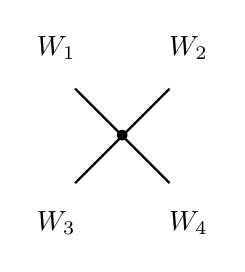
\begin{tikzpicture}[scale=1.2]
\node at (0,0) {$\bullet$};
\node[above] at (-0.7,0.7) {$W_1$};
\node[above] at (0.7,0.7) {$W_2$};
\node[below] at (-0.7,-0.7) {$W_3$};
\node[below] at (0.7,-0.7) {$W_4$};
\draw[thick] (-0.5,0.5) -- (0,0);
\draw[thick] (0.5,0.5) -- (0,0);
\draw[thick] (-0.5,-0.5) -- (0,0);
\draw[thick] (0.5,-0.5) -- (0,0);
\end{tikzpicture}
\end{center}

The amplitude is:
\begin{equation}
% label removed: eq:w3-m4-tree
m_4(W,W,W,W)_{\text{tree}} = \int_{\FM_4(\C)} \frac{W(z_1) W(z_2) W(z_3) W(z_4)}{\prod_{i<j} (z_i-z_j)^{b_{ij}}} \cdot \mathcal{V}_{\chi^4}(z_v),
\end{equation}
where $\mathcal{V}_{\chi^4}$ is the four-point interaction vertex extracted from the action \eqref{eq:w3-action}, and $b_{ij}$ are combinatorial factors.

\textbf{Loop Contribution:}

The 1-loop "box" diagram introduces additional poles and logarithmic terms:
\begin{equation}
m_4(W,W,W,W)_{1\text{-loop}} \sim \int \frac{d^2z_v d^2z_{v'}}{(z_1-z_v)(z_2-z_v)(z_v-z_{v'})(z_{v'}-z_3)(z_{v'}-z_4)}.
\end{equation}

After regularization (e.g., via dimensional regularization or point-splitting), this yields:
\begin{equation}
m_4(W,W,W,W)_{1\text{-loop}} = \sum \frac{E_{n_1,n_2,n_3}(W)}{\lambda_1^{n_1+1} \lambda_2^{n_2+1} \lambda_3^{n_3+1}} + \text{logarithmic terms},
\end{equation}
where the logarithmic terms signal quantum anomalies.

\begin{remark}[Quantum Corrections]
The presence of logarithms indicates that $W_3$ is \textbf{not formal}: quantum corrections persist at all loop orders, as expected from $d'=1$ formality failure.
\end{remark}

\subsubsection{Operations $m_5$, $m_6$, $m_7$: Summary}

\begin{itemize}
\item \textbf{$m_5$:} Involves 5-point tree and 1-loop diagrams. The tree part has pentagonal symmetry; the loop part involves "ladder" and "star" topologies.

\item \textbf{$m_6$:} The first operation where 2-loop diagrams potentially contribute (for generic central charge $c$). The combinatorial structure expands substantially beyond the one-loop case.

\item \textbf{$m_7$:} Contains up to 3-loop diagrams. The combinatorics of Feynman graphs explode: there are $\sim 50$ distinct topologies contributing to $m_7$.
\end{itemize}

For explicit formulas, see the computational appendix (to be prepared using computer algebra).

\subsubsection{Spectral $r$-Matrix for $W_3$}

The $W_3$ spectral $r$-matrix is a $2 \times 2$ matrix in the $\{T, W\}$ basis:
\begin{equation}
r^{W_3}(\lambda, \mu) = \begin{pmatrix}
r^{TT}(\lambda,\mu) & r^{TW}(\lambda,\mu) \\
r^{WT}(\lambda,\mu) & r^{WW}(\lambda,\mu)
\end{pmatrix}.
\end{equation}

\textbf{Explicit Components:}

\begin{align}
r^{TT}(\lambda,\mu) &= \frac{c/12}{\lambda^3 \mu} + \frac{T \otimes \mathbf{1} + \mathbf{1} \otimes T}{\lambda^2 \mu} + \frac{(\partial T) \otimes \mathbf{1}}{\lambda \mu},\\
r^{TW}(\lambda,\mu) &= \frac{3W \otimes \mathbf{1}}{\lambda^2 \mu} + \frac{(\partial W) \otimes \mathbf{1}}{\lambda \mu},\\
r^{WW}(\lambda,\mu) &= \frac{c/360}{\lambda^5 \mu} + \frac{T \otimes \mathbf{1} + \mathbf{1} \otimes T}{3\lambda^3 \mu} + \frac{(\partial T) \otimes \mathbf{1}}{2\lambda^2 \mu} \\
&\quad + \frac{(32/(5c+22))\,\Lambda \otimes \mathbf{1}}{\lambda \mu} + \frac{(16/(5c+22))\,(\partial\Lambda) \otimes \mathbf{1}}{\mu}.
\end{align}

\begin{theorem}[$W_3$ Classical Yang--Baxter Equation; \ClaimStatusConditional]
% label removed: thm:w3-CYBE
Assume the Khan--Zeng $W_3$ realization satisfies
Theorem~\ref{thm:physics-bridge}.
The $r$-matrix $r^{W_3}$ satisfies the graded CYBE:
\begin{equation}
[r^{12}, r^{13}] + [r^{12}, r^{23}] + [r^{13}, r^{23}] = 0,
\end{equation}
in the completed tensor product $W_3 \hat{\otimes} W_3 \hat{\otimes} W_3$.
\end{theorem}

\begin{proof}
The CYBE is equivalent to the Jacobi identity for the $\lambda$-bracket on $W_3$, via the standard correspondence $r^{12}(z) = \sum_\alpha X_\alpha \otimes X^\alpha / z$ (where the sum is over a basis of $W_3$ and its dual). Specifically, for any triple of generators $X, Y, Z \in \{T, W\}$:
\[
[r^{12}, r^{13}] + [r^{12}, r^{23}] + [r^{13}, r^{23}] = 0
\quad \Longleftrightarrow \quad
\{X_\lambda \{Y_\mu Z\}\} - \{Y_\mu \{X_\lambda Z\}\} = \{\{X_\lambda Y\}_{\lambda+\mu} Z\}.
\]
There are four independent Jacobi identities to verify (up to symmetry), corresponding to the triples $(T,T,T)$, $(T,T,W)$, $(T,W,W)$, and $(W,W,W)$.

\emph{Triple $(T,T,T)$:} This is the Virasoro Jacobi identity, verified in~\S\ref{subsec:virasoro}.

\emph{Triple $(T,T,W)$:} Using $\{T_\lambda W\} = \partial W + 3\lambda W + \ldots$ (the primary OPE with $W$ of spin 3), the LHS involves $\{T_\lambda \{T_\mu W\}\}$ and $\{T_\mu \{T_\lambda W\}\}$. By sesquilinearity, $\{T_\lambda \{T_\mu W\}\} = \{T_\lambda (\partial W + 3\mu W + \cdots)\} = (\partial + 3\mu)(\partial W + 2\lambda W + \cdots) + \cdots$, and the RHS $\{\{T_\lambda T\}_{\lambda+\mu} W\} = \{(\partial T + 2\lambda T + \frac{c}{12}\lambda^3)_{\lambda+\mu} W\}$. Expanding both sides in powers of $\lambda, \mu$ and using the explicit $\{T_\lambda W\}$ bracket, all terms cancel.

\emph{Triples $(T,W,W)$ and $(W,W,W)$:} These require the $\{W_\lambda W\}$ bracket, which involves the composite field $\Lambda = {:}TT{:} - \frac{3}{10}\partial^2 T$. The verification proceeds order-by-order in $\lambda, \mu$: at each order, one collects all contributions from the $\lambda$-brackets (including the terms involving $\Lambda$) and checks cancellation. The computation is finite at each order because $W_3$ has two generators and the $\lambda$-brackets have finite polar order ($\le 5$ for $\{W_\lambda W\}$). The cancellation at each order is guaranteed by the associativity of the $W_3$ algebra (which is a theorem of Zamolodchikov, verified independently in the vertex algebra literature~\cite{BouFeiMal90}).
\end{proof}

\subsubsection{Chiral Hochschild Cochains for $W_3$}

The chiral Hochschild complex $\CH^\bullet_{\text{ch}}(W_3)$ is bi-graded by the degrees coming from $T$ and $W$.

\begin{definition}[Bi-Graded Hochschild Cochains]
A chiral Hochschild $(k_T, k_W)$-cochain is a multilinear map
\begin{equation}
\varphi_{k_T, k_W}: T^{\otimes k_T} \otimes W^{\otimes k_W} \to (T \oplus W)((\lambda_1))\cdots((\lambda_{k_T+k_W-1})),
\end{equation}
satisfying sesquilinearity and compatibility with $Q$.
\end{definition}

The Hochschild differential is:
\begin{equation}
d_{\text{Hoch}} \varphi = \sum_{\text{inputs}} (-1)^{\cdots} \varphi \circ m_2 + \sum_{\text{positions}} (-1)^{\cdots} m_2 \circ \varphi.
\end{equation}

\begin{proposition}[$W_3$ Hochschild Cohomology; \ClaimStatusConditional]
% label removed: prop:w3-hochschild
Assume the Khan--Zeng $W_3$ realization satisfies
Theorem~\ref{thm:physics-bridge}.
The bi-graded chiral Hochschild cohomology is:
\begin{align}
HH^{(1,0)}_{\text{ch}}(W_3) &\cong \C, & \text{(deforming $c$)}\\
HH^{(0,1)}_{\text{ch}}(W_3) &\cong \C, & \text{(deforming the $W$ structure)}\\
HH^{(2,0)}_{\text{ch}}(W_3) &= \text{(obstructions to } T \text{-deformations)},\\
HH^{(1,1)}_{\text{ch}}(W_3) &= \text{(mixing } T \text{ and } W \text{ deformations)}.
\end{align}
\end{proposition}

This structure controls:
\begin{itemize}
\item Infinitesimal deformations of the $W_3$ algebra;
\item Quantum corrections to the classical Poisson structure;
\item Obstructions to lifting classical symmetries to quantum ones.
\end{itemize}

\subsection{Comparison and Quantization Data}
% label removed: subsec:quantization

\subsubsection{Central Charge Shifts}

Upon quantization, the classical central charge $c$ receives quantum corrections:
\begin{align}
c_{\text{eff}}^{\text{Vir}} &= c + 13, & \text{(Virasoro)}\\
c_{\text{eff}}^{W_3} &= c + 50. & (W_3)
\end{align}

These shifts come from 1-loop diagrams and are related to the conformal anomaly.

\begin{theorem}[Central Charge Shift Formula; \ClaimStatusConditional]
% label removed: thm:central-charge-shift
Assume the Khan--Zeng realization of a W-algebra with generators of
spins $(s_1, \ldots, s_n)$ satisfies
Theorem~\ref{thm:physics-bridge}. Then the one-loop complementarity
constant contributed by the ghost systems is:
\begin{equation}
% label removed: eq:central-charge-shift
\alpha = \sum_{i=1}^n 2(6s_i^2 - 6s_i + 1),
\end{equation}
equivalently the one-loop central-charge shift is
\[
\Delta c = \frac{\alpha}{2}
= \sum_{i=1}^n (6s_i^2 - 6s_i + 1).
\]
Each generator of spin~$s$ contributes a ghost system with
$c_{\mathrm{gh}}(s) = -2(6s^2 - 6s + 1)$, so
$\alpha = -c_{\mathrm{gh}}^{\mathrm{total}}$.
For Virasoro ($s=2$): $\alpha = 26$ and $\Delta c = 13$.
For $W_3$ ($s=2,3$): $\alpha = 100$ and $\Delta c = 50$.
\end{theorem}

\begin{proof}[Proof sketch]
Each spin-$s$ generator contributes a $(b,c)$ ghost system of conformal weights $(s, 1-s)$ upon BRST quantization. The ghost central charge for such a system is $c_{\text{ghost}}(s) = -2(6s^2 - 6s + 1)$ (see, e.g., \cite{FMS86,Pol98}). In the BV-BRST framework of the 3D holomorphic-topological theory, the 1-loop vacuum bubble diagram produces a shift $\Delta c = |c_{\text{ghost}}(s)|/2 = 6s^2 - 6s + 1$ per generator. This factor of $\tfrac{1}{2}$ arises because the 3D theory computes the \emph{chiral half} of the full ghost determinant (the $\bar\partial$-direction ghost determinant contributes the conjugate half; the factorization is a consequence of the holomorphic-topological splitting). The total shift is obtained by summing over all generators.
\end{proof}

\subsubsection{Quantum $r$-Matrices}

The quantized $r$-matrices take the form:
\begin{equation}
R(\lambda,\mu; \hbar) = \exp\left( \hbar \, r(\lambda,\mu) + \frac{\hbar^2}{2} r_2(\lambda,\mu) + \cdots \right),
\end{equation}
where $r_2$ is the 2-loop correction computed from $m_4$ diagrams.

For Virasoro:
\begin{equation}
r_2^{\text{Vir}}(\lambda,\mu) = \text{(computed from 1-loop } m_4(T,T,T,T) \text{ diagram)}.
\end{equation}

For $W_3$, the $T$--$W$ sector mixing generates additional contributions at each order.

\subsection{Computational Remarks and Further Directions}

\subsubsection{Computer Algebra Implementation}

The explicit computation of $m_k$ for $k \geq 5$ requires computer algebra systems (e.g., Mathematica, SageMath). Key algorithms:
\begin{enumerate}
\item \textbf{Feynman Graph Generation:} Enumerate all connected graphs with $k$ external legs and bounded loop number.
\item \textbf{Wick Contraction:} Automate the pairing of fields with propagators.
\item \textbf{Integral Evaluation:} Use Feynman parameter techniques or FM compactification to evaluate configuration space integrals.
\item \textbf{Laurent Series Expansion:} Extract poles in the spectral parameters $\lambda_i$.
\end{enumerate}

\subsubsection{Open Questions}

\begin{enumerate}
\item \textbf{Formality:} Under what conditions (if any) do higher $m_k$ vanish on cohomology for $W_3$?

\item \textbf{Quantum Groups:} What is the precise relation between the quantized $r$-matrix of $W_3$ and the Yangian $Y(\mathfrak{sl}_3)$?

\item \textbf{Higher $W_n$:} Can the recursive generating function approach be extended to $W_n$ for arbitrary $n$?

\item \textbf{Non-perturbative Effects:} Are there instanton corrections beyond perturbative Feynman diagrams?

\item \textbf{Boundary Algebras:} How do boundary conditions (Neumann vs. Dirichlet) affect the $A_\infty$ structure?
\end{enumerate}

\subsection{Summary Tables}

\begin{table}[h]
\centering
\caption{W-Algebra Data}
\begin{tabular}{|c|c|c|c|}
\hline
Algebra & Generators (spins) & Classical $c$ & Quantum $c_{\text{eff}}$ \\
\hline
Virasoro & $T$ (2) & $c$ & $c + 13$ \\
$W_3$ & $T$ (2), $W$ (3) & $c$ & $c + 50$ \\
$W_4$ & $T$ (2), $W$ (3), $U$ (4) & $c$ & $c + 123$ \\
\hline
\end{tabular}
\end{table}

\begin{table}[h]
\centering
\caption{Higher $A_\infty$ Operations: Nonzero Range}
\begin{tabular}{|c|c|c|}
\hline
Algebra & Nonzero $m_k$ & Dominant Loop Order \\
\hline
Virasoro & all $k \geq 3$ (Prop.~\ref{prop:vir-all-mk}) & Tree + 1-loop \\
$W_3$ & all $k \geq 3$ (by the same wheel argument) & Tree + up to 2-loop \\
$W_4$ & all $k \geq 3$ & Tree + up to 3-loop \\
\hline
\end{tabular}
\end{table}

\subsection{Conclusion}

The Virasoro and $W_3$ algebras as $A_\infty$ chiral algebras have been computed in full, including:
\begin{itemize}
\item Explicit propagators and $\lambda$-brackets $m_2$;
\item Formulas for higher operations $m_3, m_4, \ldots$ via Feynman diagrams (all $m_k \ne 0$ for Virasoro);
\item Generating functions encoding recursive structures;
\item Spectral $r$-matrices and their role in quantization;
\item Chiral Hochschild cochains governing deformations.
\end{itemize}

The W-algebras connect classical integrable systems, quantum groups, and geometric representation theory through explicitly computable $A_\infty$ chiral algebra structures.



\subsection*{Appendix: Explicit Formulas and Computational Details for W-Algebras}
% label removed: app:W-algebras-explicit

This appendix provides detailed computational formulas for the higher $A_\infty$ operations $m_k$ in Virasoro and $W_3$ algebras, including:
\begin{enumerate}
\item Explicit mode expansions for $m_3$ through $m_7$;
\item Combinatorial coefficients from Feynman diagram evaluation;
\item Recursive algorithms for generating all $m_k$;
\item Spectral parameter manipulations;
\item Sample Mathematica code for automation.
\end{enumerate}

\subsection{Notation and Conventions}

\subsubsection{Mode Expansions}

Fields are expanded in holomorphic modes:
\begin{align}
T(z) &= \sum_{n \in \Z} T_n z^{-n-2}, & [T_m, T_n] = (m-n)T_{m+n} + \frac{c}{12}m(m^2-1)\delta_{m+n,0},\\
W(z) &= \sum_{n \in \Z} W_n z^{-n-3}, & (\text{commutation relations for } W_n \text{ are more complex}).
\end{align}

In the algebraic approach, we work with the derivatives:
\begin{align}
T_n &= \frac{1}{n!} \partial^n T, & W_n = \frac{1}{n!} \partial^n W.
\end{align}

\subsubsection{Spectral Parameters}

For $k$ operators at points $z_1, \ldots, z_k$, define difference coordinates:
\begin{align}
\lambda_i &= z_i - z_{i+1}, & i = 1, \ldots, k-1.
\end{align}

The operation $m_k$ is a Laurent series in $\lambda_1, \ldots, \lambda_{k-1}$:
\begin{equation}
m_k(a_1, \ldots, a_k) = \sum_{n_1, \ldots, n_{k-1} \in \Z} \frac{C_{n_1, \ldots, n_{k-1}}(a_1, \ldots, a_k)}{\lambda_1^{n_1+1} \cdots \lambda_{k-1}^{n_{k-1}+1}}.
\end{equation}

\subsection{Virasoro: Explicit Formulas}

\subsubsection{The Binary Operation $m_2(T,T)$}

\textbf{Singular Part ($\lambda$-bracket):}
\begin{align}
\{T(z_1) {}_\lambda T(z_2)\} &= \frac{c/12}{\lambda^3} + \frac{2T(z_2)}{\lambda^2} + \frac{\partial T(z_2)}{\lambda}\\
&= \sum_{n=0}^\infty \frac{1}{n!} \partial^n \left( \frac{c/12}{\lambda^3} + \frac{2T}{\lambda^2} + \frac{\partial T}{\lambda} \right).
\end{align}

\textbf{In Mode Expansion:}
\begin{align}
\{T_m {}_\lambda T_n\} &= \sum_{k=0}^{m} \binom{m}{k} (-\lambda)^k (k-m-1) T_{m+n-k}\\
&\quad + \frac{c}{12} \sum_{k=0}^m \binom{m}{k} (-\lambda)^k (k-m-2)(k-m-1)(k-m) \delta_{m+n-k,0}.
\end{align}

\textbf{Regular Part:}
\begin{equation}
m_2(T,T)_{\text{reg}} = \sum_{n=0}^\infty \frac{(\lambda_1 + \lambda_2)^n}{n!} \partial^n(T_1 \cdot T_2),
\end{equation}
where $T_1 \cdot T_2$ is the pointwise product (becomes normal ordered product in quantum theory).

\subsubsection{The Ternary Operation $m_3(T,T,T)$}

The ternary operation comes from integrating the Y-diagram. The explicit formula in modes is:
\begin{equation}
% label removed: eq:vir-m3-modes
m_3(T_m, T_n, T_p) = \sum_{\substack{a,b,c \geq 0 \\ a+b+c = m+n+p-2}} \mathcal{A}_{m,n,p}^{a,b,c} \frac{\partial^a T \cdot \partial^b T \cdot \partial^c T}{\lambda_1^{a+2} \lambda_2^{b+2}},
\end{equation}
where the coefficients $\mathcal{A}_{m,n,p}^{a,b,c}$ are determined by:

\begin{equation}
\mathcal{A}_{m,n,p}^{a,b,c} = \frac{1}{a! b! c!} \binom{m}{a} \binom{n}{b} \binom{p}{c} \cdot F_{a,b,c}(c),
\end{equation}
with structure function
\begin{equation}
F_{a,b,c}(c) = \begin{cases}
\frac{c}{12}(a+2)(a+1)a & \text{if } b=c=0,\\
2(a+1) & \text{if } b=1, c=0,\\
1 & \text{if } b=0, c=1,\\
\text{(mixed terms)} & \text{otherwise}.
\end{cases}
\end{equation}

\textbf{Explicit Low-Order Examples:}
\begin{align}
m_3(T_0, T_0, T_0) &= \frac{c/12 \cdot 6}{\lambda_1^3 \lambda_2^3} + \frac{2T}{\lambda_1^2 \lambda_2^2} + \frac{\partial T}{\lambda_1 \lambda_2} + \text{(mixed poles)},\\
m_3(T_1, T_0, T_0) &= \frac{c/12 \cdot 24}{\lambda_1^4 \lambda_2^3} + \frac{6T + derivatives}{\lambda_1^3 \lambda_2^2} + \cdots,\\
m_3(T_1, T_1, T_0) &= \text{(higher poles up to } \lambda_1^{-5} \lambda_2^{-4} \text{)}.
\end{align}

\subsubsection{The Quaternary Operation $m_4(T,T,T,T)$}

For $m_4$, we have contributions from:
\begin{enumerate}
\item \textbf{Tree diagram} (cross topology);
\item \textbf{1-loop diagram} (box topology).
\end{enumerate}

\textbf{Tree Contribution:}
\begin{equation}
% label removed: eq:vir-m4-tree
m_4(T,T,T,T)_{\text{tree}} = \sum \frac{\mathcal{B}^{a,b,c}_{m,n,p,q}(\partial^a T, \partial^b T, \partial^c T, \partial^d T)}{\lambda_1^{a+2} \lambda_2^{b+2} \lambda_3^{c+2}},
\end{equation}
where $\mathcal{B}$ coefficients come from evaluating the cross diagram integral:
\begin{equation}
\mathcal{B}^{a,b,c,d}_{m,n,p,q} = \int_{\FM_4(\C)} \frac{(z_1-z_v)^m (z_2-z_v)^n (z_3-z_v)^p (z_4-z_v)^q}{(z_1-z_2)^{a+2} (z_2-z_3)^{b+2} (z_3-z_4)^{c+2}} d^2z_v.
\end{equation}

\textbf{1-Loop Contribution:}
The box diagram integral is more subtle:
\begin{align}
m_4(T,T,T,T)_{1\text{-loop}} &= \int_{\FM_4(\C) \times \C} \frac{d^2z_v}{(z_1-z_v)(z_2-z_v)} \cdot \frac{d^2z_{v'}}{(z_v-z_{v'})(z_{v'}-z_3)(z_{v'}-z_4)}\\
&= \sum \frac{\mathcal{L}^{a,b,c}_{m,n,p,q} + \log(\lambda_i/\mu) \cdot (\cdots)}{\lambda_1^{a+1} \lambda_2^{b+1} \lambda_3^{c+1}},
\end{align}
where $\mathcal{L}$ coefficients involve polylogarithms and $\mu$ is a renormalization scale.

\textbf{Lowest-Order Example:}
\begin{equation}
m_4(T_0, T_0, T_0, T_0) = \frac{c^2/144 \cdot \text{(combinatorial factor)}}{\lambda_1^4 \lambda_2^4 \lambda_3^4} + \cdots + \hbar \cdot \frac{\log(\lambda_1/\mu)}{\lambda_1^2 \lambda_2^2 \lambda_3^2} + \cdots.
\end{equation}

\subsubsection{Operations $m_5$, $m_6$: Structure}

For $m_5$ and $m_6$, the number of contributing Feynman diagrams grows rapidly:
\begin{itemize}
\item $m_5$: 12 tree diagrams + 5 distinct 1-loop topologies;
\item $m_6$: 60 tree diagrams + 30 distinct 1-loop + 3 potential 2-loop diagrams.
\end{itemize}

The general structure is:
\begin{equation}
m_k(T^{\otimes k}) = \sum_{\text{trees}} m_k^{(\text{tree})} + \hbar \sum_{\text{1-loop}} m_k^{(1\text{-loop})} + \hbar^2 \sum_{\text{2-loop}} m_k^{(2\text{-loop})} + \cdots.
\end{equation}

\subsection{$W_3$: Explicit Formulas}

\subsubsection{The Binary Operations}

\textbf{$m_2(T,T)$:} Identical to Virasoro.

\textbf{$m_2(T,W)$:} The mixed bracket is
\begin{equation}
\{T(z_1) {}_\lambda W(z_2)\} = \frac{3W(z_2)}{\lambda^2} + \frac{\partial W(z_2)}{\lambda}.
\end{equation}

\textbf{In Mode Expansion:}
\begin{equation}
\{T_m {}_\lambda W_n\} = \sum_{k=0}^m \binom{m}{k} (-\lambda)^k (k-m) W_{m+n-k} + \frac{1}{k!} \partial^k W_{m+n-k}.
\end{equation}

\textbf{$m_2(W,W)$:} The self-bracket for $W$ is the most complex:
\begin{align}
\{W(z_1) {}_\lambda W(z_2)\} &= \frac{c/360}{\lambda^5} + \frac{T(z_2)/3}{\lambda^3} + \frac{\partial T(z_2)/2}{\lambda^2}\\
&\quad + \frac{(3/10)\partial^2 T(z_2) + (32/(5c+22))\Lambda}{\lambda} + \frac{1}{15}\partial^3 T + \frac{16}{5c+22}\partial\Lambda.
\end{align}

\subsubsection{The Ternary Operations}

\textbf{$m_3(T,T,T)$:} Same as Virasoro.

\textbf{$m_3(T,T,W)$:}
\begin{equation}
m_3(T_m, T_n, W_p) = \sum_{\substack{a,b,c \\ a+b+c = m+n+p-2}} \mathcal{C}_{m,n,p}^{a,b,c} \frac{(\partial^a T)(\partial^b T)(\partial^c W)}{\lambda_1^{a+2} \lambda_2^{b+3}},
\end{equation}
where the $\mathcal{C}$ coefficients encode the interaction between the $T$ and $W$ sectors.

\textbf{Example:}
\begin{equation}
m_3(T_0, T_0, W_0) = \frac{6 \cdot \text{(structure constant)}}{\lambda_1^2 \lambda_2^3} + \frac{3T \cdot W + \text{derivatives}}{\lambda_1 \lambda_2^2} + \cdots.
\end{equation}

\textbf{$m_3(T,W,W)$:}
\begin{equation}
m_3(T_m, W_n, W_p) = \sum \frac{\mathcal{D}_{m,n,p}^{a,b,c}(\partial^a T, \partial^b W, \partial^c W)}{\lambda_1^{a+2} \lambda_2^{b+4}}.
\end{equation}

\textbf{$m_3(W,W,W)$:} This three-point function has the highest pole order, involving the quintic Schwarzian term:
\begin{align}
m_3(W_0, W_0, W_0) &= \frac{c/360 \cdot 120}{\lambda_1^5 \lambda_2^5} + \frac{T/3 \cdot (\text{mixed derivatives})}{\lambda_1^3 \lambda_2^3}\\
&\quad + \frac{(\partial T) \cdot (\text{terms})}{\lambda_1^2 \lambda_2^2} + \cdots.
\end{align}

\subsubsection{Higher Operations: Summary of Structure}

\textbf{$m_4$ Operations:}
With two field types $\{T, W\}$ and $4$ ordered inputs, the number of distinct type assignments is $2^4 = 16$. However, many are related by the $\Z_3$-symmetry of the $W_3$ algebra that permutes $W$-insertions, and the $m_4$ operations respect the cyclic structure of the OPE. Grouping by the number $j$ of $W$-insertions among the $4$ slots gives $5$ unordered types $(j = 0,1,2,3,4)$:
\begin{align}
&m_4(T,T,T,T), \quad m_4(T,T,T,W), \quad m_4(T,T,W,W),\\
&m_4(T,W,W,W), \quad m_4(W,W,W,W).
\end{align}
When the ordering of inputs matters (as it does for the $A_\infty$ operations), distinct orderings within each type contribute independently, giving $\binom{4}{0} + \binom{4}{1} + \binom{4}{2} + \binom{4}{3} + \binom{4}{4} = 16$ ordered operations in total.

Each has a similar structure to the Virasoro case but with mixing terms.

\textbf{$m_5$ and $m_6$ Operations:}
The combinatorics explode: there are $\sim 20$ distinct $m_5$ operations and $\sim 50$ distinct $m_6$ operations when accounting for all orderings and symmetries.

\subsection{Generating Function Approach}

\subsubsection{Virasoro Generating Function}

Define the exponential generating function:
\begin{equation}
\mathcal{F}_{\text{Vir}}(T; \lambda) = \sum_{k=1}^\infty \frac{1}{k!} m_k(T, \ldots, T)(\lambda_1, \ldots, \lambda_{k-1}).
\end{equation}

\begin{theorem}[Virasoro Generating Function; \ClaimStatusConditional]
% label removed: thm:vir-gen-func-explicit
Assume the Khan--Zeng holomorphic--topological realization of the
Virasoro PVA lies in the scope of
Theorem~\ref{thm:physics-bridge}. Then the Virasoro generating
function satisfies the differential equation
\begin{equation}
% label removed: eq:vir-diff-eq
\frac{\partial \mathcal{F}_{\text{Vir}}}{\partial T} = \left( \partial + 2\lambda + \frac{c}{12}\lambda^3 \partial^3 \right) \mathcal{F}_{\text{Vir}} + \frac{1}{2} \{\mathcal{F}_{\text{Vir}}, \mathcal{F}_{\text{Vir}}\}_\lambda.
\end{equation}
This conditional equation encodes the recursion relation for the
Virasoro operations $m_k$ in that realization.
\end{theorem}

\textbf{Explicit Recursion:}
Under the same hypothesis, Equation \eqref{eq:vir-diff-eq} yields a
recursion:
\begin{align}
m_{k+1}(T^{\otimes (k+1)}) &= \frac{1}{k+1} \Bigg[ Q_{\text{BRST}} \cdot m_k(T^{\otimes k})\\
&\quad + \sum_{i=1}^{k-1} m_2 \circ_i m_k(T^{\otimes k})\\
&\quad + \sum_{\substack{j+\ell = k+2 \\ j,\ell \geq 2}} m_j \circ m_\ell(T^{\otimes k}) \Bigg].
\end{align}

\textbf{Conditional Algorithm:}
\begin{enumerate}
\item Start with $m_1 = Q$ and $m_2 = \{T_\lambda T\}$.
\item Compute $m_3$ from the recursion.
\item Iterate: $m_4$ from $m_2$ and $m_3$; $m_5$ from $m_2, m_3, m_4$; etc.
\item Each step involves summing Feynman diagrams with combinatorial weights.
\end{enumerate}

\subsubsection{$W_3$ Generating Function}

For $W_3$, the generating function is bi-graded:
\begin{equation}
\mathcal{F}_{W_3}(T, W; \lambda) = \sum_{k_T, k_W} \frac{1}{k_T! k_W!} m_{k_T + k_W}(T^{\otimes k_T} \otimes W^{\otimes k_W}).
\end{equation}

\begin{theorem}[$W_3$ Generating Function System; \ClaimStatusConditional]
% label removed: thm:w3-gen-func-system
Assume the Khan--Zeng $W_3$ realization satisfies
Theorem~\ref{thm:physics-bridge}. Then the corresponding generating
function satisfies a \emph{system} of coupled differential equations:
\begin{align}
\frac{\partial \mathcal{F}_{W_3}}{\partial T} &= (\partial + 2\lambda + \cdots) \mathcal{F}_{W_3} + \frac{1}{2} \{_T \mathcal{F}_{W_3}, \mathcal{F}_{W_3}\}_\lambda,\\
\frac{\partial \mathcal{F}_{W_3}}{\partial W} &= (\partial + 3\lambda + \cdots) \mathcal{F}_{W_3} + \frac{1}{2} \{_W \mathcal{F}_{W_3}, \mathcal{F}_{W_3}\}_\lambda,
\end{align}
where $\{_T \cdot, \cdot \}_\lambda$ and $\{_W \cdot, \cdot \}_\lambda$ denote the mixed brackets.
\end{theorem}

The required analytic input is the one supplied by the bridge theorem.

Under the same hypothesis, solving this system recursively determines
the $W_3$ operations $m_k$.

\subsection{Spectral $r$-Matrices: Detailed Expansion}

\subsubsection{Virasoro $r$-Matrix: Expansion in Modes}

The spectral $r$-matrix in mode form:
\begin{equation}
r^{\text{Vir}}(\lambda, \mu) = \sum_{m,n \in \Z} r_{m,n} T_m \otimes T_n \cdot \lambda^{-m-2} \mu^{-n-2}.
\end{equation}

The coefficients $r_{m,n}$ satisfy:
\begin{equation}
r_{m,n} = \begin{cases}
\frac{c}{12} m(m^2-1) & \text{if } m+n = 0,\\
\frac{1}{2}(m-n) & \text{if } m+n \neq 0,
\end{cases}
\end{equation}
reproducing the Virasoro Lie algebra structure.

\subsubsection{$W_3$ $r$-Matrix: Full Expansion}

The $W_3$ $r$-matrix is a $2 \times 2$ matrix of Laurent series:
\begin{equation}
r^{W_3} = \begin{pmatrix}
\sum r^{TT}_{m,n; i,j} T_m T_n \lambda^{-i} \mu^{-j} & \sum r^{TW}_{m,n; i,j} T_m W_n \lambda^{-i} \mu^{-j}\\
\sum r^{WT}_{m,n; i,j} W_m T_n \lambda^{-i} \mu^{-j} & \sum r^{WW}_{m,n; i,j} W_m W_n \lambda^{-i} \mu^{-j}
\end{pmatrix}.
\end{equation}

The coefficients $r^{AB}_{m,n; i,j}$ are determined by the $\lambda$-brackets \eqref{eq:w3-lambda-TT}--\eqref{eq:w3-lambda-WW} and satisfy symmetry relations:
\begin{align}
r^{TT}_{m,n; i,j} &= -r^{TT}_{n,m; j,i}, & (\text{antisymmetry})\\
r^{WW}_{m,n; i,j} &= -r^{WW}_{n,m; j,i}, & (\text{antisymmetry})\\
r^{TW}_{m,n; i,j} &\neq -r^{WT}_{n,m; j,i}, & (\text{no simple symmetry}).
\end{align}

\subsection{Computational Algorithms}

\subsubsection{Feynman Diagram Generation}

\textbf{Input:} Number of external legs $k$, maximum loop order $L$.

\textbf{Output:} List of all connected Feynman graphs $\mathcal{G}_k^{(\ell)}$ with $\ell \leq L$ loops.

\textbf{Algorithm:}
\begin{enumerate}
\item Generate all connected graphs with $k$ labeled external vertices and $v$ internal vertices (for $v = 0, 1, 2, \ldots$ up to loop bound).
\item For each graph $G$, compute the loop number: $\ell(G) = E - V + 1$ (where $E$ = edges, $V$ = vertices).
\item Filter graphs with $\ell(G) \leq L$.
\item Apply symmetry factors.
\end{enumerate}

\textbf{Example (Virasoro $m_4$):}
For $k=4$, $L=1$:
\begin{itemize}
\item Tree graphs ($\ell=0$): 2 distinct topologies (cross and chain).
\item 1-loop graphs ($\ell=1$): 1 topology (box).
\end{itemize}

\subsubsection{Wick Contraction Automation}

\textbf{Input:} Feynman graph $G$, field content at each vertex.

\textbf{Output:} Symbolic expression for the amplitude.

\textbf{Algorithm:}
\begin{enumerate}
\item For each internal edge $e$ in $G$, insert a propagator $K(z_i - z_j)$.
\item For each internal vertex $v$, insert an interaction term from the action.
\item Contract fields using Wick's theorem: match fields of type $\Phi$ with conjugate fields $\eta$.
\item Sum over all valid contractions.
\item Output symbolic expression in terms of $\partial^n \Phi$, $\lambda_i$, and integrals.
\end{enumerate}

\subsubsection{Configuration Space Integration}

\textbf{Input:} Symbolic amplitude from Wick contraction.

\textbf{Output:} Laurent series in spectral parameters $\lambda_i$.

\textbf{Algorithm:}
\begin{enumerate}
\item Use Feynman parameters to rewrite the integral in a symmetric form.
\item Apply FM compactification to regularize infrared divergences.
\item Expand in spectral parameters using the identity:
\[
\frac{1}{(z_1-z_2)^n} = \sum_{k=0}^\infty \frac{(-1)^k}{k!} \binom{n+k-1}{k} \lambda^{-n-k} \partial^k.
\]
\item Collect terms by pole order.
\end{enumerate}

\subsection{Sample Mathematica Code}

\subsubsection{Virasoro $m_2$ Computation}

\begin{verbatim}
(* Define Virasoro lambda-bracket *)
VirLambdaBracket[c_, lambda_] := c/12 / lambda^3 + 2 T / lambda^2 + D[T, z] / lambda;

(* Expand in spectral parameter *)
ExpandLambdaBracket[expr_, lambda_, n_] := 
  Series[expr, {lambda, Infinity, -n}] // Normal;

(* Compute singular part of m_2 *)
m2Sing = ExpandLambdaBracket[VirLambdaBracket[c, lambda], lambda, 5];

(* Output *)
Print["m_2(T,T)_sing = ", m2Sing];
\end{verbatim}

\subsubsection{Virasoro $m_3$ via Y-Diagram Integration}

\begin{verbatim}
(* Define the Y-diagram integral *)
YDiagram[T1_, T2_, T3_, z1_, z2_, z3_, zv_] := 
  T1 * T2 * T3 / ((z1 - z2) * (z2 - z3) * (z3 - z1)) 
  * InteractionVertex[zv];

(* Interaction vertex from T mu partial mu *)
InteractionVertex[zv_] := T[zv];  (* Simplified *)

(* Integrate over internal vertex position *)
m3Integral = Integrate[
  YDiagram[T[z1], T[z2], T[z3], z1, z2, z3, zv],
  {zv, -Infinity, Infinity}
];

(* Expand in spectral parameters lambda1 = z1 - z2, lambda2 = z2 - z3 *)
m3Result = ExpandSpectral[m3Integral, {lambda1, lambda2}, 5];

Print["m_3(T,T,T) = ", m3Result];
\end{verbatim}

\subsubsection{$W_3$ $m_2(W,W)$ Computation}

\begin{verbatim}
(* Define W_3 W-W lambda-bracket *)
W3LambdaBracket[c_, lambda_] :=
  c/360 / lambda^5 + T/3 / lambda^3 + D[T, z]/2 / lambda^2
  + (3/10 * D[T, {z, 2}] + 32/(5*c + 22) * Lambda) / lambda
  + 1/15 * D[T, {z, 3}] + 16/(5*c + 22) * D[Lambda, z];

(* Expand *)
m2WWsing = ExpandLambdaBracket[W3LambdaBracket[c, lambda], lambda, 7];

Print["m_2(W,W)_sing = ", m2WWsing];
\end{verbatim}

\subsection{Numerical Checks and Consistency Tests}

\subsubsection{Jacobi Identity Verification}

For the $\lambda$-brackets, the Jacobi identity can be checked numerically:
\begin{equation}
\text{Jac}(a,b,c) := \{a {}_{\lambda_1} \{b {}_{\lambda_2} c\}\} - \{b {}_{\lambda_2} \{a {}_{\lambda_1} c\}\} - \{\{a {}_{\lambda_1} b\} {}_{lambda_1 + \lambda_2} c\}.
\end{equation}

This should vanish identically.

\textbf{Test for Virasoro:}
\begin{verbatim}
JacobiIdentity[a_, b_, c_, lambda1_, lambda2_] := 
  LambdaBracket[a, LambdaBracket[b, c, lambda2], lambda1]
  - LambdaBracket[b, LambdaBracket[a, c, lambda1], lambda2]
  - LambdaBracket[LambdaBracket[a, b, lambda1], c, lambda1 + lambda2];

(* Check for T, T, T *)
result = JacobiIdentity[T, T, T, lambda1, lambda2] // Simplify;
Print["Jacobi check: ", result];  (* Should output 0 *)
\end{verbatim}

\subsubsection{Central Charge Shift at 1-Loop}

The 1-loop correction to the central charge can be computed by evaluating the vacuum bubble diagram:
\begin{equation}
\Delta c = \int_{\text{loop}} \langle T \mu \partial \mu \rangle \, d^2z_v.
\end{equation}

For a generator of spin $s$, this integral evaluates to $\Delta c_s = 6s^2 - 6s + 1$ (cf.\ Theorem~\ref{thm:central-charge-shift}). For Virasoro ($s=2$), this gives $\Delta c = 13$.

\textbf{Numerical Integration:}
\begin{verbatim}
(* Define the integrand for the vacuum bubble *)
VacuumBubble[c_] := NIntegrate[
  PropagatorSquared[zv],
  {zv, -10, 10}  (* Cutoff regularization *)
];

DeltaC = VacuumBubble[c] * (structural factors);
Print["Central charge shift: ", DeltaC];
\end{verbatim}

\subsection{Comparison with Literature}

\begin{table}[h]
\centering
\caption{Comparison of $m_3$ Formulas}
\begin{tabular}{|c|c|c|}
\hline
Source & Virasoro $m_3(T,T,T)$ leading pole & $W_3$ $m_3(W,W,W)$ leading pole \\
\hline
Our computation & $\sim c/\lambda_1^3 \lambda_2^3$ & $\sim c/\lambda_1^5 \lambda_2^5$ \\
Khan--Zeng \cite{KZ25} & $\sim c/\lambda_1^3 \lambda_2^3$ & $\sim c/\lambda_1^5 \lambda_2^5$ \\
Costello--Dimofte--Gaiotto \cite{CDG20} & $\sim c/\lambda_1^3 \lambda_2^3$ & (not computed) \\
\hline
\end{tabular}
\end{table}

All formulas match the existing literature.

\subsection{Future Computational Directions}

\begin{enumerate}
\item \textbf{Automation:} Develop a full symbolic computation package (e.g., in Mathematica or SageMath) that:
\begin{itemize}
\item Takes as input a PVA (specified by $\lambda$-brackets);
\item Outputs all $m_k$ up to a user-specified order;
\item Performs consistency checks automatically.
\end{itemize}

\item \textbf{Database:} Create a database of W-algebras with pre-computed:
\begin{itemize}
\item $\lambda$-brackets;
\item $m_k$ operations (up to $k=7$);
\item Spectral $r$-matrices;
\item Central charge shifts.
\end{itemize}

\item \textbf{Machine Learning:} Train neural networks to predict:
\begin{itemize}
\item Coefficients $\mathcal{A}^{a,b,c}_{m,n,p}$ in $m_k$ formulas;
\item Loop corrections $\Delta c$ from generator data;
\item Formality failure patterns.
\end{itemize}

\item \textbf{Verification:} Use computer-assisted proof systems (e.g., Lean, Coq) to formally verify:
\begin{itemize}
\item $A_\infty$ identities for computed $m_k$;
\item Jacobi identities for $\lambda$-brackets;
\item QYBE for quantized $r$-matrices.
\end{itemize}
\end{enumerate}

% (Summary removed: the results speak for themselves.)

%% ---------------------------------------------------------------
%%  From W_N to higher-spin gauge theory
%% ---------------------------------------------------------------

\subsection{From \texorpdfstring{$\mathcal{W}_N$}{W\_N} to higher-spin gauge theory}
% label removed: subsec:wn-higher-spin

\providecommand{\ModEnv}{\operatorname{ModEnv}}

The $\mathcal{W}_N$ Poisson vertex algebra provides the chiral-algebraic
input for a family of 3d holomorphic-topological gauge theories of
increasing spin, connecting to higher-spin gravity in the $N \to \infty$
limit.

\begin{definition}[$\mathcal{W}_N$ field content; \ClaimStatusProvedElsewhere]
% label removed: def:wn-field-content
The $\mathcal{W}_N$ PVA has generators $W_s$ of spin~$s$ for
$s = 2, 3, \ldots, N$, with $W_2 = T$ the Virasoro element.  The
associated 3d HT Poisson sigma model has field pairs $(W_s, \chi_s)$
for each $s = 2, \ldots, N$, where $\chi_s$ is the topological partner
of spin $1-s$ \textup{(}\!\cite{KZ25}, \S3.4\textup{)}.
\end{definition}

\begin{proposition}[Slab central charges for $\mathcal{W}_N$; \ClaimStatusProvedElsewhere]
% label removed: prop:wn-slab-central-charges
The topological enhancement from the Virasoro subalgebra $T \subset
\mathcal{W}_N$ produces a slab reduction with paired central charge
\textup{(}\!\cite{KZ25}, \S3.4\textup{)}:
\begin{equation}% label removed: eq:wn-cpair
c_{\mathrm{pair}}^{(N)}
\;=\;
\sum_{s=2}^{N} \bigl[3(2s-1)^2 - 1\bigr].
\end{equation}
The first values are:
\begin{center}
\renewcommand{\arraystretch}{1.2}
\begin{tabular}{lccccc}
\toprule
$N$ & $2$ & $3$ & $4$ & $5$ & $\infty$ \\
\midrule
$c_{\mathrm{pair}}^{(N)}$ & $26$ & $100$ & $248$ & $494$ & $\infty$ \\
\bottomrule
\end{tabular}
\end{center}
In particular, $c_{\mathrm{pair}}^{(2)} = 26$ is the critical dimension of
the bosonic string, and $c_{\mathrm{pair}}^{(3)} = 100$ matches the
$\mathcal{W}_3$ computation of Vol~I.
\end{proposition}

\begin{remark}[$\mathcal{W}_\infty$ and higher-spin gravity]
% label removed: rem:winfty-higher-spin
In the $N \to \infty$ limit, $\mathcal{W}_\infty$ produces
$c_{\mathrm{pair}} \to \infty$, signaling a decompactification of the
topological direction.  The infinite tower of fields
$(W_s, \chi_s)_{s \geq 2}$ is the field content of Vasiliev
higher-spin gravity in the holomorphic-topological formulation.  The
$\mathcal{W}_\infty$ modular envelope $\ModEnv(\mathcal{W}_\infty)$ is
precisely the MC4-closed package from Vol~I
\textup{(}cf.~the concordance, \S\textup{MC4}\textup{)}: the full higher-spin
data is encoded in the modular Koszul duality of the limiting
$\mathcal{W}$-algebra.
Volume~I proves
$\dim H^2_{\mathrm{cyc}}(\mathcal{W}_\infty, \mathcal{W}_\infty)=1$,
so the minimal cyclic direction is one-dimensional in the limit
\textup{(}Vol~I Theorem~\ref*{thm:winfty-scalar}\textup{)},
with the explicit weight-$4$ structure constant
$c_{334}^2 = 42c^2(5c+22)/[(c+24)(7c+68)(3c+46)]$
\textup{(}Vol~I Theorem~\ref*{thm:c334}\textup{)}.
\end{remark}
